\documentclass[a4paper, 11pt]{article}
\usepackage[utf8]{inputenc}
%\usepackage[ansinew]{inputenc}

\usepackage{geometry}
\usepackage{amsmath}
\usepackage{amssymb}
\usepackage{graphicx}
\usepackage{color}
\usepackage{verbatim}
\usepackage{subfig}

\newcommand{\code}[1]{\texttt{#1}}
\newcommand{\codeex}[2][0.98\textwidth]{\vspace*{1ex}\noindent\fbox{\parbox{#1}{\verbatiminput{#2}}}\vspace*{1ex}}
\newcommand{\todo}[1]{\textcolor{red}{\textsc{ToDo:} #1}}
\newcommand{\DerWeg}{\textit{DerWeg }} % the blank space is important!
\newcommand{\AnicarViewer}{\textit{AnicarViewer }} % the blank space is important!

\geometry{
body={16cm, 24.7cm},
left=2.5cm,
top=2.5cm
}

\title{Overview of Hardware and Software for the Cognitive Automobile Lab}
\author{Dr. Martin Lauer, Dipl.-Ing. Bernd Kitt}
\date{11. April 2011}

\begin{document}\sloppypar{
\maketitle

\tableofcontents

\section{Hardware}

\subsection{AniCar}
This vehicle was, with the exception of some components, completely designed by the MRT (Institut fuer Mess- und Regelungstechnik). The vehicle was designed in such a way, that it fulfills the requirements of the cognitive automobile laboratory and allows for a simple operation.  Operation is initialized in three steps:
\begin{itemize}
\item{Establish voltage supply (switch batteries on and connect them to the vehicle)}
\item{Connect components (Cameras)}
\item{Connect laptop (USB, Ethernet)}
\end{itemize}
All electrical ports in the vehicle, as well as all cables connected to it, are labeled. Labeling allows for easy and understandable cabling. A plug mix-up is not possible. 
\begin{figure}[htb]
\centering
\captionsetup[subfloat]{nearskip = -3pt}
\subfloat[Complete Overview]{\includegraphics[width=75mm]{anicar}\label{fig:anicar}}\quad
\subfloat[Details]{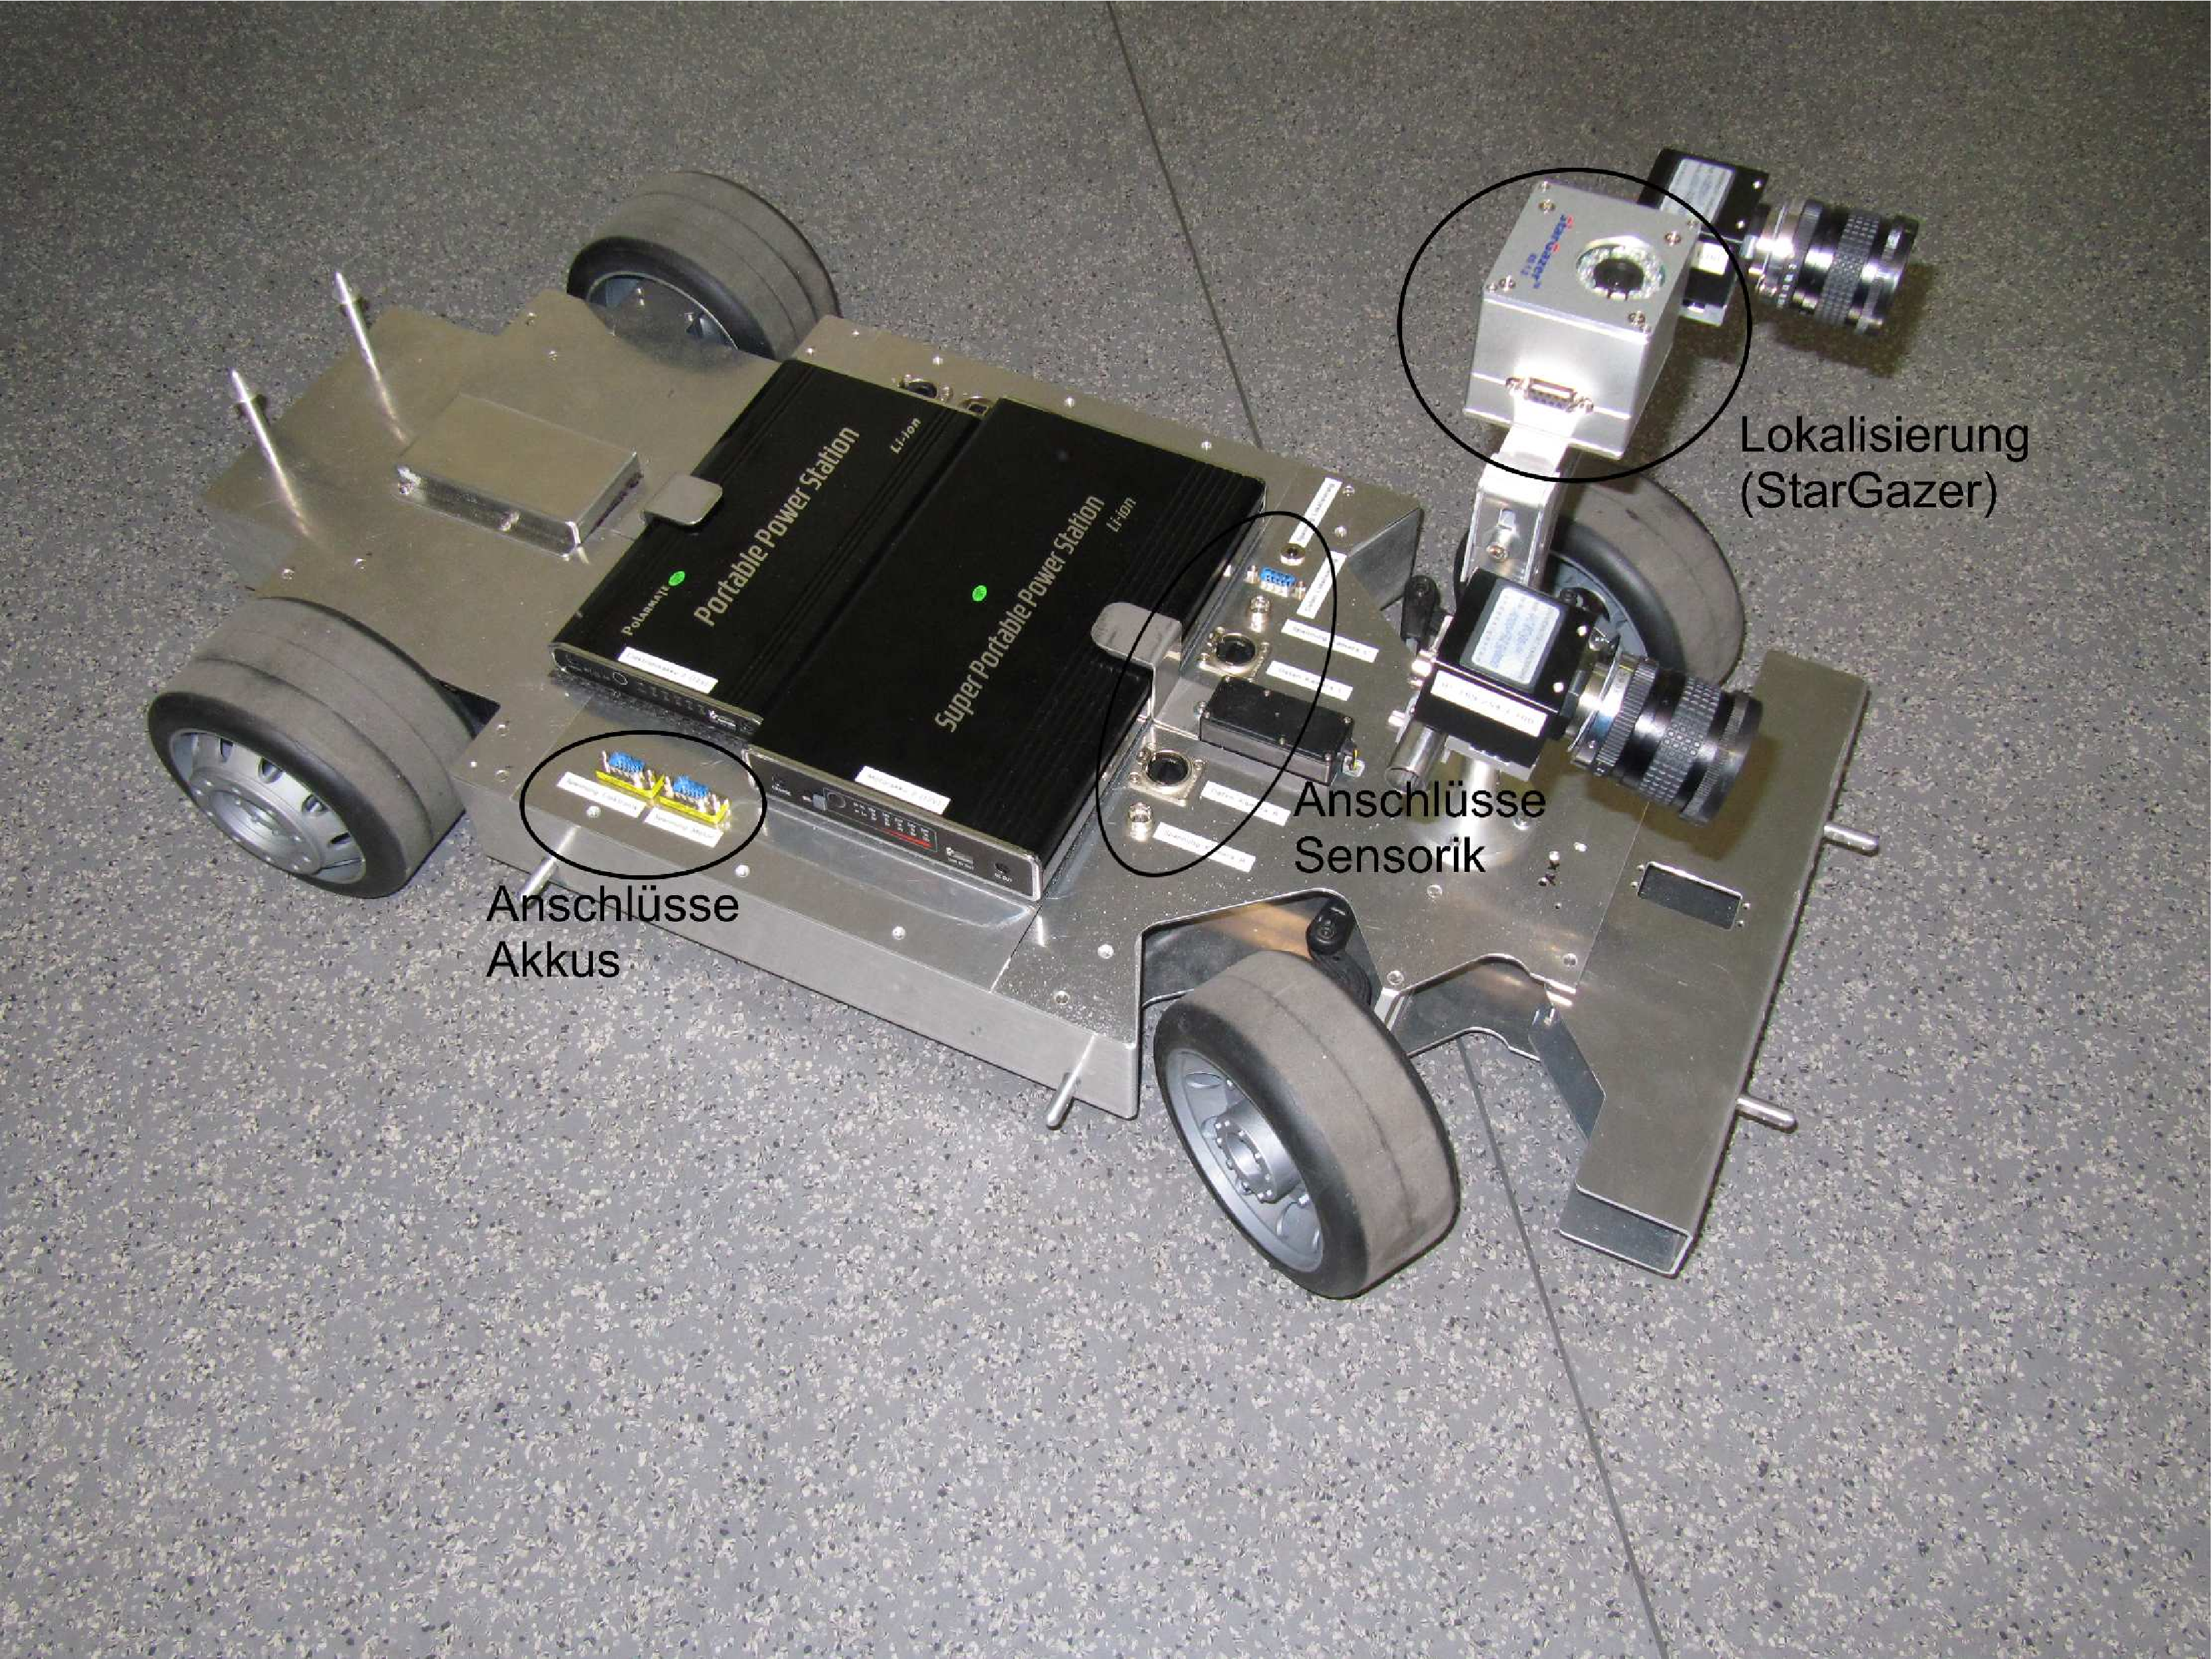
\includegraphics[width=75mm]{anicarSensors}\label{fig:sensors}}
\captionof{figure}[]{AniCar}
\label{fig:anicarImage}
\end{figure}
Only the supervisor may open the vehicle. Nonetheless, students are allowed to replace the batteries.

\subsection{Batteries}
The batteries can be switched on and off by holding a button (electronic battery), and with help from a switch (motor battery). The button also aids in setting the voltage (by holding the button until the LED starts blinking, then releasing). Shortly pushing the button displays the current charging level of the battery. The small battery is responsible for all electronic components, while the larger battery takes care of the motor. Given that both work with the same voltage, mixing up the connectors does not cause any damage.\\ 
\newline
Notes:
\begin{itemize}
\item{Please turn all batteries off after every use.}
\item{\textbf{Batteries should be operated with 12 V! (Switch on "`Lo"').}}
\end{itemize}

% \subsection{Localization (StarGazer)}
% The \textit{StarGazer} is a localization system for indoor robots. It is works using landmarks mounted on different corners. These landmarks are beamed at by infrared LEDs mounted on the StarGazer. Reflected light is recorded by a camera\footnote{Given the infrared component of sunlight, some disruptions in the localization are expected. For that reason, active landmarks are employed, which emit IR-light themselves. This leads to a significantly more reliable localization.} Based on these images, it is possible to determine the position and orientation of the vehicle (StarGazer) relative to a given landmark.  The conversion of “landmark coordinates” into global “course coordinates” has already been implemented. With this, a provided pose can be directly portrayed in the course. 
\subsection{Localization}
The vehicle’s self-localization works based on the landmarks placed on the corners and on a upward facing camera mounted on the vehicle. The landmarks are equipped with infrared LEDs. These diodes define a landmark’s ID as well as a local coordinate system in it. The upward facing camera detects the landmarks and with that information, determines the vehicle’s position as well as its orientation.

\subsection{Cameras}
Regarding cameras, color cameras with gigabit-ethernet connection are employed. This allows for frame rates up to 200 fps, depending on the used resolution.

\section{Vehicle Control program \DerWeg}

The vehicle’s behavior is determined within the \DerWeg control program, and is initialized on the AniCar computer. The program gathers feed from the vehicle’s sensors (camera, localization system, odometry), controls the drivetrain and steering motors, and analyses camera imaging. It then calculates an appropriate behavior for a given situation and regulates speed and steering angle. A framework program, which defines the communication with the sensors and motor enabling, is provided by the lab. Image analysis and behavior generation and regulation on the other side, must be added.  Only some demo applications have been implemented at this point. (see section \ref{sec:modules}).

\subsection{Software structure}

The program \DerWeg was designed as a modular concept and follows a so-called \textit{Blackboard architecture}.  This means that the software contains some modules that are independent from each other. All modules have access to the Blackboard. From there, they can read and write information on the vehicle's status and sensors. Therefore, all information exchange between modules occurs exclusively through the Blackboard. Figure \ref{fig:blackboardArchitecture} illustrates this setup.

All individual modules are independent threads. This means each module has a function \code{execute()}, which runs almost parallel to every other module. Even though the different modules are not actually time-synchronized, the blackboard works around by using mutual exclusion (mutex) and conditional variables. This allows to some extent for a synchronization of the modules and safe access to the blackboard thread.

\begin{figure}
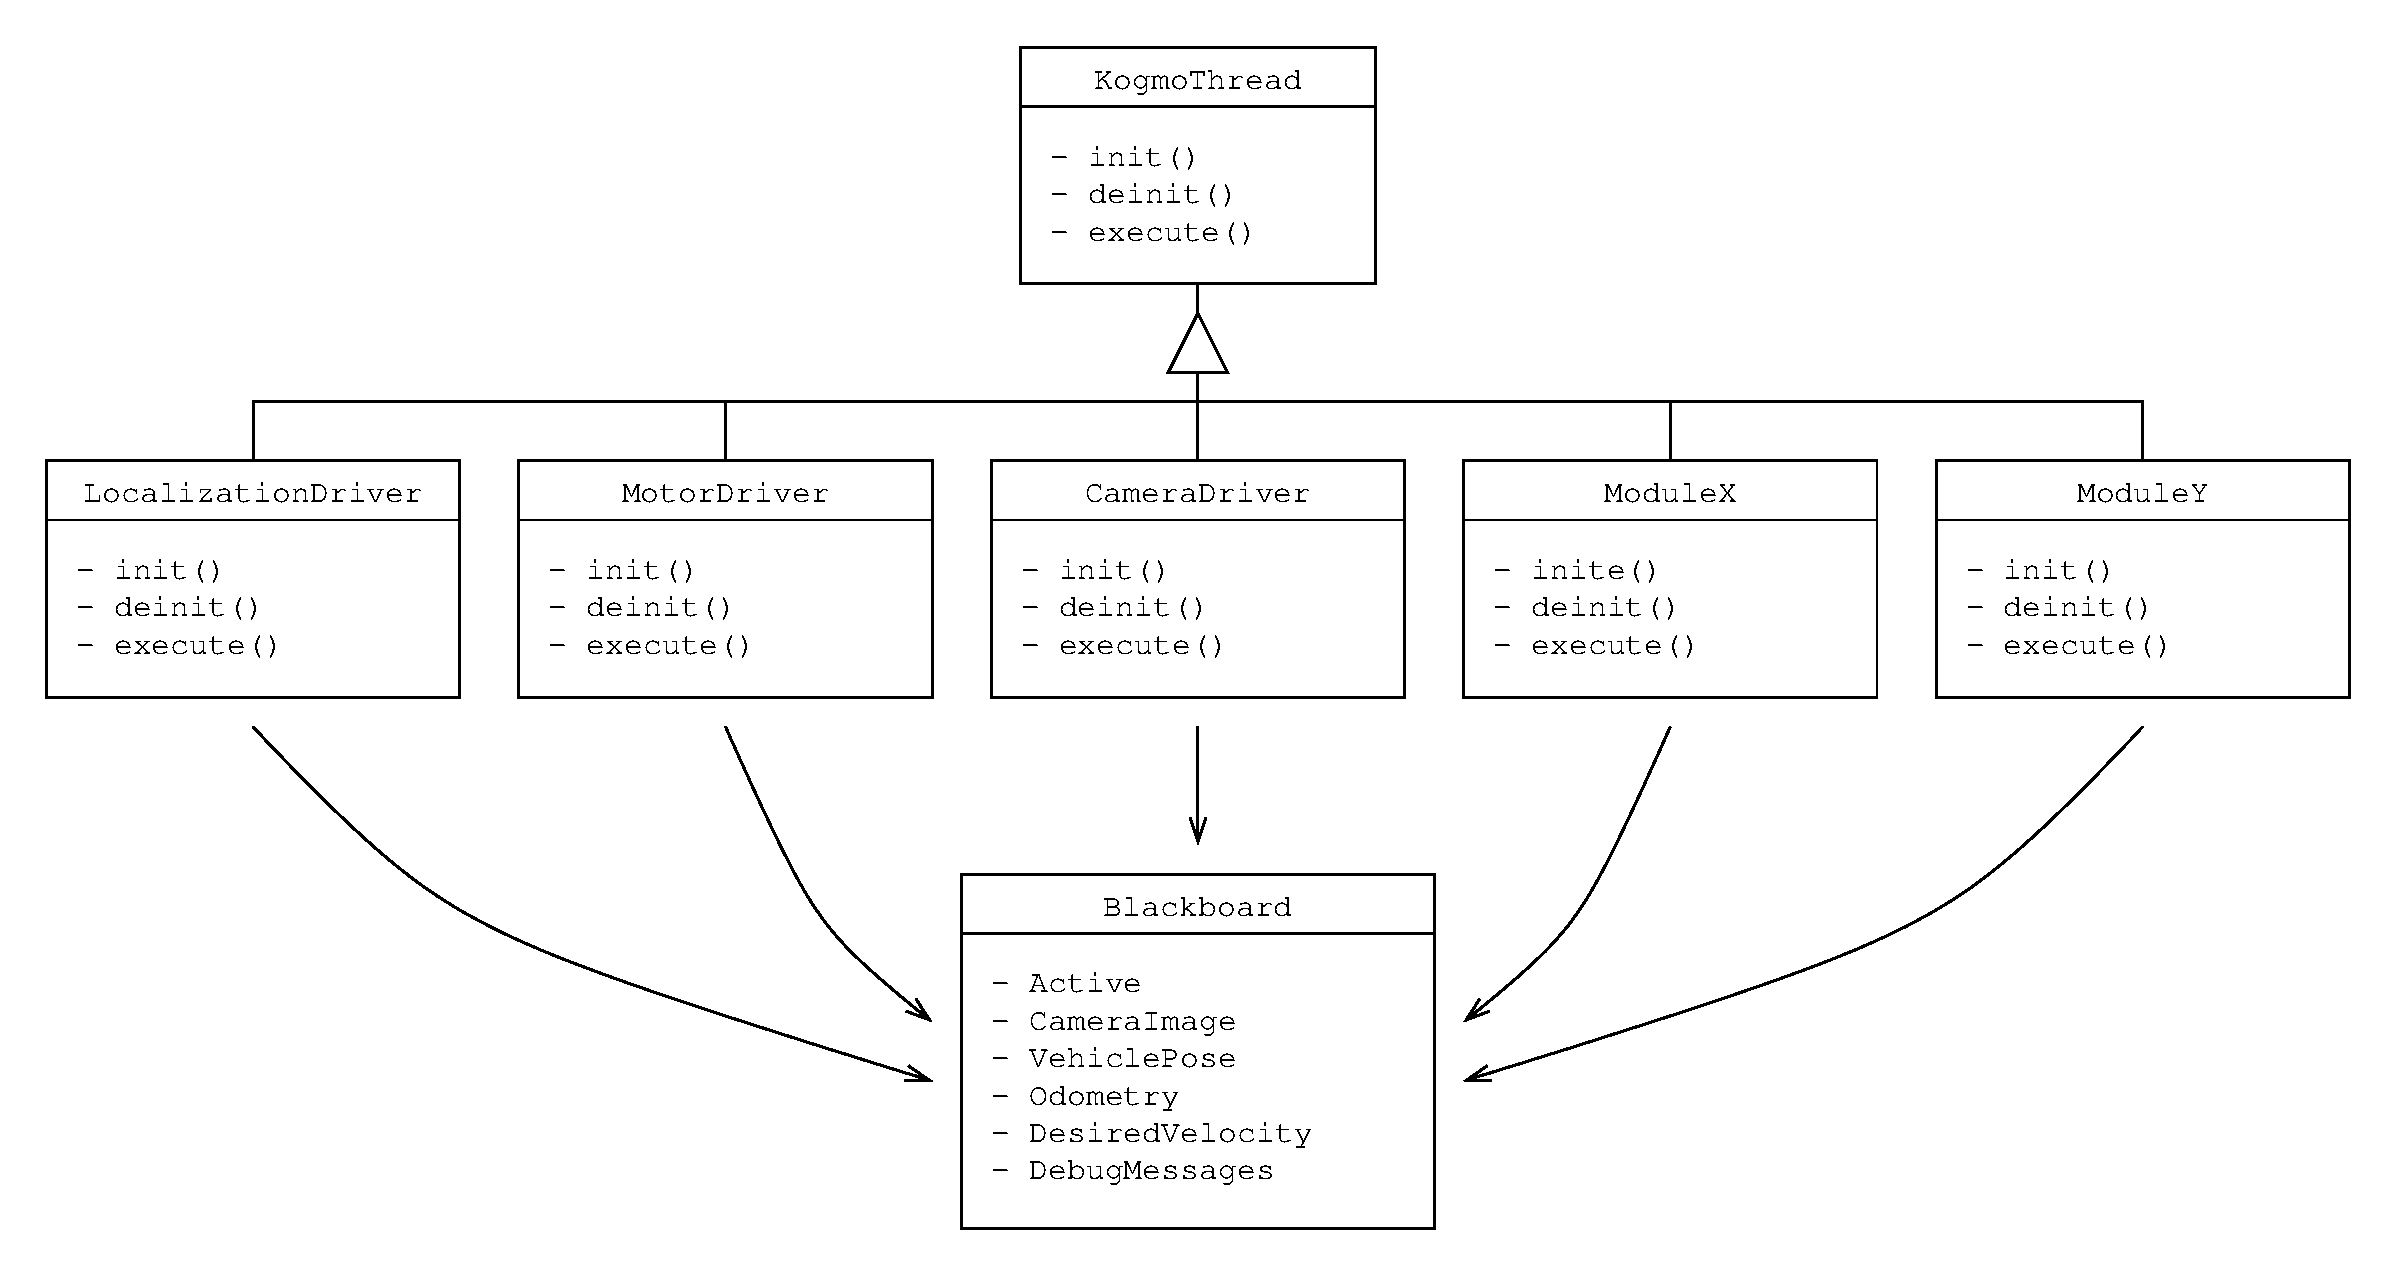
\includegraphics[width=\textwidth]{blackboardArchitecture}
\caption{Blackboard architecture schematics. All modules are independent threads, derived from the class \code{Kogmothread}. They retrieve all relevant information from the blackboard and consequently deliver their results there. There is no direct coupling between modules.}
\end{figure}

\subsubsection{The Blackboard}
The Blackboard is an object to which all modules have access. It contains essentially the following information:
\begin{itemize}
\item Vehicle status (activated/deactivated)
\item Position, orientation, speed, and yaw angle. (Speed and yaw angle are calculated based on the most recently measured vehicle position).
\item Vehicle odometry (speed measured at the wheels as well as steering angle)
\item The desired speed and angle.
\item The current camera image.
\end{itemize}

Access to the blackboard is simple. For every available piece of information, there are three methods of accessing (See Annex \ref{app:blackboard}):
\begin{itemize}
\item \code{X getX ()} delivers information of type X ($X\in \{ \text{Active}, \text{VehiclePose}, \text{Odometry},\linebreak \text{DesiredVelocity}, \text{Image} \}$)
\item \code{void setX (X)} overwrites the information in the blackboard.
\item \code{bool waitForX (time\_duration)} stops the requesting function from running until new information of type X is available, or until a predefined, maximum time interval has elapsed (default 1s). It delivers \textit{true} when new information has been found, and \textit{false} when the given time has elapsed without gaining new information.
\end {itemize}

\paragraph{Example}
If the user wishes to read the current vehicle pose from the blackboard with a function \code{f()} and also set a desired speed, then the program would look like this:

\codeex{beispielBlackboard.cpp}


\subsection{Modules}
All modules in the program \DerWeg are independent threads. The are derived from a common parent class \code{KogmoThread} and provided the following interface:
\begin{itemize}
\item Function \code{init()} initializes the module.
\item Function \code{deinit()} deinitializes the module.
\item Function \code{execute()} actually puts the module into action, and is started as an independent thread.
\end{itemize}

A thread acts like an independent program within the main program. The \code{execute()} function plays the role that a typical \code{main()} would in C++. Therefore, \code{execute()} takes care of controlling flow. In our case, it will be generally written as an infinite loop.

\paragraph{Example}
A module’s \code{execute()} function that repeatedly displays the current vehicle pose on a screen, could be built in the following way:

\codeex{beispielModulEinfach.cpp}

As the example shows, the \code{execute()} function is run as an infinite loop. This means, the function will never stop computing by itself. Therefore, it is important to interrupt the loop “from the outside”, with the code allowing to do so written inside of it.

This is possible with help from the \code{boost::this\_thread::interruption\_point()} function, which defines a so-called “cancellation point”.

How do cancellation points work? If a thread B wishes to interrupt another thread A, it sends a so-called cancellation request. Thread A does not react to it initially, but waits until it hits a cancellation point. Once it arrives , A checks for pending cancellation requests. If there are none, then the program continues running. Otherwise, if there is a request at hand, the program is interrupted and a \code{boost::thread\_interrupted} exception is thrown. At this point, all subsequent instructions in the running program are skipped until a \code{catch(boost::thread\_interrupted\&)} line is found. From that point, the program will continue running normally. 

In the example there is a cancellation point defined within the infinite loop. If the thread (here the \code{execute()}) function) is prompted to cancel, and the program reaches the cancellation point, then the execution of the program will be interrupted, it will be jumped to the Catch-Block, and then will go on working underneath the catch-block . Given that our example has no more code written under the catch-block, the end of the \code{execute()} function will be immediately reached, and the thread will terminate.

The \code{init()} and \code{deinit()} functions allow for variable initialization, as well as allocation and freeing of memory space and resources; they work similar to a constructor and destructor. It often happens, that some parameter values are given to a module from a start in order to influence its mode of operation. For example, a camera driver must know if the camera should be started in black and white or in color mode. 
Image processing algorithms need specific parameters ,(such as threshold values), which should preferably not be written (fixed) in the main code. 

To achieve this, the \code{init()} function is given an object of type \code{ConfigReader} as an argument. This object reads a configuration file during program startup and evaluates it. Parameter values are listed in this file according to the key-value-principle. This means, each parameter possesses a keyword and each keyword is assigned a value. When the value of a parameter with a given keyword “X” is read, then the ConfigReader is asked for it by using its \code{get()} functions.

\codeex{Example}
The following code reads the \textit{GigE::color\_space}, \textit{GigE::gain} and \textit{GigE::image\_size} parameters from the \code{ConfigReader}:

\codeex{beispielConfigReaderAnfrage.cpp}

As it has been pointed out, the \code{get()} function gets two arguments: the parameter’s keyword and a reference to the variable where the \code{get()} function stores the value of the parameter. The second variable can be of the \code{string, int, unsigned int, float, double} or \code{bool} types depending on which kind of parameter is requested. Aside from that, it is possible to obtain arrays of values. To accomplish this, a variable of the \code{vector$<$int$>$, vector$<$double$>$}, etc type must be given, acting as the second argument. The \code{get()} function will return a \code{true} when the sought key has been found, and a \code[false} when none are found. The design of the configuration file is described in more detail under section \ref{sec:config}.

\subsubsection{Module Manager}
The software’s module manager follows a plugin concept that allows for easy addition of new modules. If the user wishes to add a new module to the software, the following steps should be followed:
\begin{enumerate}
\item Derive a new class from the \code{KogmoThread} class:

\codeex[0.9\textwidth]{beispielModulAbleiten.cpp}

\item Register the new module in the module manager and give it a unique name, under which it will later be found. (here “MeinNeuesModul”):

\codeex[0.9\textwidth]{beispielModulAnmelden.cpp}

\item Recompile the \DerWeg software.
\end{enumerate}
 Following these 3 steps, the new module will become available in the software. The last step before using the new module is to select it. For this, some additional items are entered in configuration file. See Section \ref{sec:config}.

\subsection{Special Classes and Structures}

\subsubsection{Image Processing}

The “image” class \code{ImageBuffer} is the class used in our software to process camera images. It can represent both black and white or color images (for stereo cameras both images), as well as their respective timestamp. For image display, the \texttt{ev:Mat} image class from the \textit{opencv} software library is used. \footnote{opencv available for versions 2.X and up}. For more information on opencv, a detailed handbook can be found online under \texttt{http://opencv.itseez.com/}. To facilitate an easy start in this library, we have listed the most important functions to access access images on opencv.

Images are stored in the \texttt{cv::Mat} class. If \textit{im} is such an object, then:
\begin{itemize}
\item \texttt{im.cols} gives the image’s width.
\item \texttt{im.rows} gives the height.
\item \texttt{im.type()} gives the image type. The following two types are relevant to us:
\begin{itemize}
\item \texttt{CV\_8UC1} Grey-value image with 256 shades of grey.
\item \texttt{CV\_8UC3} Color image with $256^3$ colors.
\end{itemize}
\item with the \texttt{at} method, individual pixels are accessed.
\begin{itemize}
\item Grey-value images: \texttt{im.at<uchar>(v,u)} delivers the grey-value of the pixel at the $v$-th row and the $u$-th column.
\item Color images: \texttt{im.at<cv::Vec3b>(v,u)} delivers the color value of the pixel at the $v$-th row and the $u$-th column. Color values are presented in RGB color space. \textbf{Warning:} The order of the R, G, and B values is reversed on opencv: The B value comes first, then the G value, and finally the R value. Hence, the color model is denoted as \textit{BGR} here. To access the values individually, use brackets:
\texttt{im.at<cv::Vec3b>(v,u)[0]} provides the B-value, \texttt{im.at<cv::Vec3b>(v,u)[1]} provides the G-value, and \texttt{im.at<cv::Vec3b>(v,u)[2]} provides the R-value.
\end{itemize}
\end{itemize}

% \subsubsection{Given function}
% \label{sec:gegebene_funktionen}
%
% Aside from the general image processing functions covered in the \textit{OpenCV} library, a rather simple function that can detect and interpret road signs is also available. This can be used as part of a project, or as a starting point for an own development project. To make use of this function within one’s own code, the \code{TrafficSignDetector.h} file must be included. Only then may the traffic sign recognition be called, using \code{std::vector<TrafficSign> signs = detector.process(Image);}. \code{struct} \textit{signs} contains a list of all detectable signs and their meaning: For instance, no entry, or turn signs).  Additionally, the list contains the size and center point of the encountered signs. 

\subsubsection{Stereo image processing}
\label{sec:stereo}

It is possible to create a depth image from a pair of images taken with a stereo camera system. That is, it is possible to determine the distance from a pixel to the camera. In order to obtain this value, we must use a disparity estimator. This process uses the computer’s graphics card and as a result works at high speed. To use it, an object of the \texttt{DerWeg::StereoGPU} class must be created. The constructor needs a configuration file that can be found in the PC under \textit{/home/common/calib.xml}. After that, the depth estimator can be used.

To use the depth estimator on a stereo image pair, two commands are needed:
\begin{itemize}
\item \texttt{tiefenschaetzer.runStereoMatching(image\_left,image\_right);} starts depth estimation for an image pair.
\item \texttt{tiefenschaetzer.getStereoResults(depth, confidence, disparity, rectified\_left);} waits for the estimation to be ready and collects the results. \textit{depth} contains the estimated depth for every pixel (expressed in meters as a float value). \textit{confidence} is the “confidence” with which the values were estimated, from 0=bad to 255=good. \textit{disparity} is the disparity, and \textit{rectified\_left} is the rectified left image. Important: The depth value of a pixel can only be considered correct when its confidence value is high, i.e. good. 
\end{itemize}

In the time between \texttt{runStereoMatching} and \texttt{getStereoResults}, the CPU may still run parallel computations. One possible intermediate computation could be to carry out the segmentation of an image, or to identify road signs or lights. The overall process looks like this:
\codeex[0.9\textwidth]{beispielStereo.cpp}

An example of working with stereo images can be found under the file \textit{Application/ShowStereoCameraImage.cpp}.

\subsubsection{Vehicle Localization and Vehicle Speed}

To describe the vehicle’s position and velocity, the \code{Velocity}, \code{Odometry}, and \code{Pose} classes are used.  The desired velocity, \code{Velocity} consists of two variables: the desired velocity in longitudinal direction (given in $\frac{m}{s}$) and the desired steering angle.  This data is used by the motor control system to regulate the driving and steering motors.

The adjusted velocity and angle are returned to \DerWeg by the motor control system, and can be read as \code{Odometry}. However, it should be noted that the odometry displays the velocity at the wheels, and not of the entire vehicle, which may differ on account of slipping. Likewise, there are a few degrees of play on the steering that may cause a small nuance between the measured angle and the actual angle.

The third important value in the vehicle pose and velocity determination scheme is the localization system, which determines the position with help from landmarks. The estimated vehicle position and orientation are presented as the \code{Pose} class. \code{Pose} comprises four attributes: The vehicle’s measured position, its orientation, the estimated longitudinal velocity, and its yaw angle. The first two values work taking the measurements of the localization system and the odometry into consideration. Generally, the position can be determined with inaccuracies smaller than a centimeter. They may grow however, once the vehicle starts distancing itself from a landmark. Once the vehicle has abandoned the course, localization is no longer possible. In this case, the position may only be updated by odometry. It should also be noted that when velocity increases, the quality of the localization decreases.

The whole process works based on a general reference coordinate system and a reference position for the vehicle. The coordinate system is drawn on the ground of the field (or \textit{Machine park}), and the reference point is measured at the middle of the vehicle’s front axle. Angles are measured counterclockwise. 

Estimations on longitudinal velocity and yaw angle are made through a one-second-interval regression process. This estimation is independent from the odometry. If the actual velocity starts lagging behind, then the vehicle will begin a gradual acceleration.

\subsubsection{Console Output}

Output in C++ is generally displayed on the console. This occurs either through the \textit{cout} and \textit{cerr} streams, or through the C command: \textit{printf}. These features are not always recommendable for multi-threads as they can lead to unforeseeable errors, particularly causing “deadlocks”, which happen when a program or individual modules freeze and stop computing. To work around this, \DerWeg implements two new macros, \textit{LOUT} and \textit{EOUT}, which assume the position of \textit{cout} and \textit{cerr}, but are thread friendly. The usage of the macros varies slightly from that of the \textit{cout} and \textit{cerr} commands. A more detailed comparison is presented in the table \ref{tab:thread_safe_logging}. To access \textit{LOUT} and \textit{EOUT}, one must first \texttt{\#include} \texttt{Blackboard.h} or \texttt{ThreadSafeLogging.h} either directly or indirectly. Otherwise, the compiler will report an error when interpreting.

\begin{table}
\centering
\begin{tabular}{|p{0.45\textwidth}|p{0.45\textwidth}|}
\hline
\multicolumn{1}{|c|}{not thread safe} & \multicolumn{1}{c|}{Thread safe } \\
\hline
\tt cout $\!<<\!$ \"{}Value=\"{} $\!<<\!$ i $\!<<\!$ endl; &
\tt LOUT (\"{}Value=\"{} $\!<<\!$ i $\!<<\!$ endl) \\
\tt cerr $\!<<\!$ \"{}Value=\"{} $\!<<\!$ i $\!<<\!$ endl; &
\tt EOUT (\"{}Value=\"{} $\!<<\!$ i $\!<<\!$ endl) \\
\tt printf (\"{}Value=\%d$\backslash$n\"{}, i); & 
\tt LOUT (\"{}Value=\"{} $\!<<\!$ i $\!<<\!$ endl) \\
\tt fprintf (stderr, \"{}Value=\%d$\backslash$n\"{}, i); & 
\tt EOUT (\"{}Value=\"{} $\!<<\!$ i $\!<<\!$ endl) \\
\hline
\end{tabular}
\caption{Comparison of text output by thread safe and thread unsafe variants in the console. All examples return the text “Value=”, followed by an integer variable \textit{i} and conclude adding a line feed.}
\label{tab:thread_safe_logging}
\end{table}

\subsection{User Interactions and Visualization Tools}

The software currently contains two modules that allow the user to interact with the vehicle. These are: a simple, text-based interaction over the console, and a graphical user interface (GUI).

\subsubsection{Text-based User Interface}
\label{sec:tui}

The software module "`TUI"' offers a text-based user interface. If this module is used when starting \DerWeg , a help text will appear. The help text describes all relevant commands that are executed after entering specific keys.  
They are:

\begin{description}
\item[q] (quit) terminates the programm execution.
\item[g] (go) activates the vehicle. At first, when the programm is initialized the vehicle is deactivated. That is, driving commands are not executed.
\item[blank] (stop) stops and deactivates the vehicle. 
\item[s] (status) displays vehicle's position and velocity. 
\item[c] (configuration) displays the loaded software modules. 
\item[h] (help) Shows the help text. 
\item[x,y,+,-] The user is allowed, under certain conditions, to use these keys to manually control the vehicle. This override is just possible when the target speed is not being influences by any other modules. 
\end{description}

\subsubsection{Graphical User Interface}
\label{sec:gui}

In addition to the TUI employed in the AniCar control computer, the software allows for a graphical user interface (GUI) with the name \AnicarViewer. \AnicarViewer is a standalone programm which communicates with \DerWeg over a network connection. The purpose of this is to enable \AnicarViewer to be started in a separate computer to \DerWeg. For example, as long as both computers are connected via a WLAN, \DerWeg can be started on the AniCar control computer, while \AnicarViewer runs on a standard computer in the computer room. Such a configuration makes it possible to control the vehicle without having to physically follow behind it. However, if the WLAN/WiFi connection is interrupted, even if just for a few seconds, the vehicle will be completely unaccessible during this period.  

The GUI is started by calling \texttt{AnicarViewer Hostname}, whereas \texttt{Hostname} represents the IP adress of the computer running \DerWeg. The designations \textit{localhost} and \textit{anicar} are also valid. Additionally, the window featured in figure \ref{fig:AnicarViewerSnapshot} will appear. 

\begin{figure}
\centering
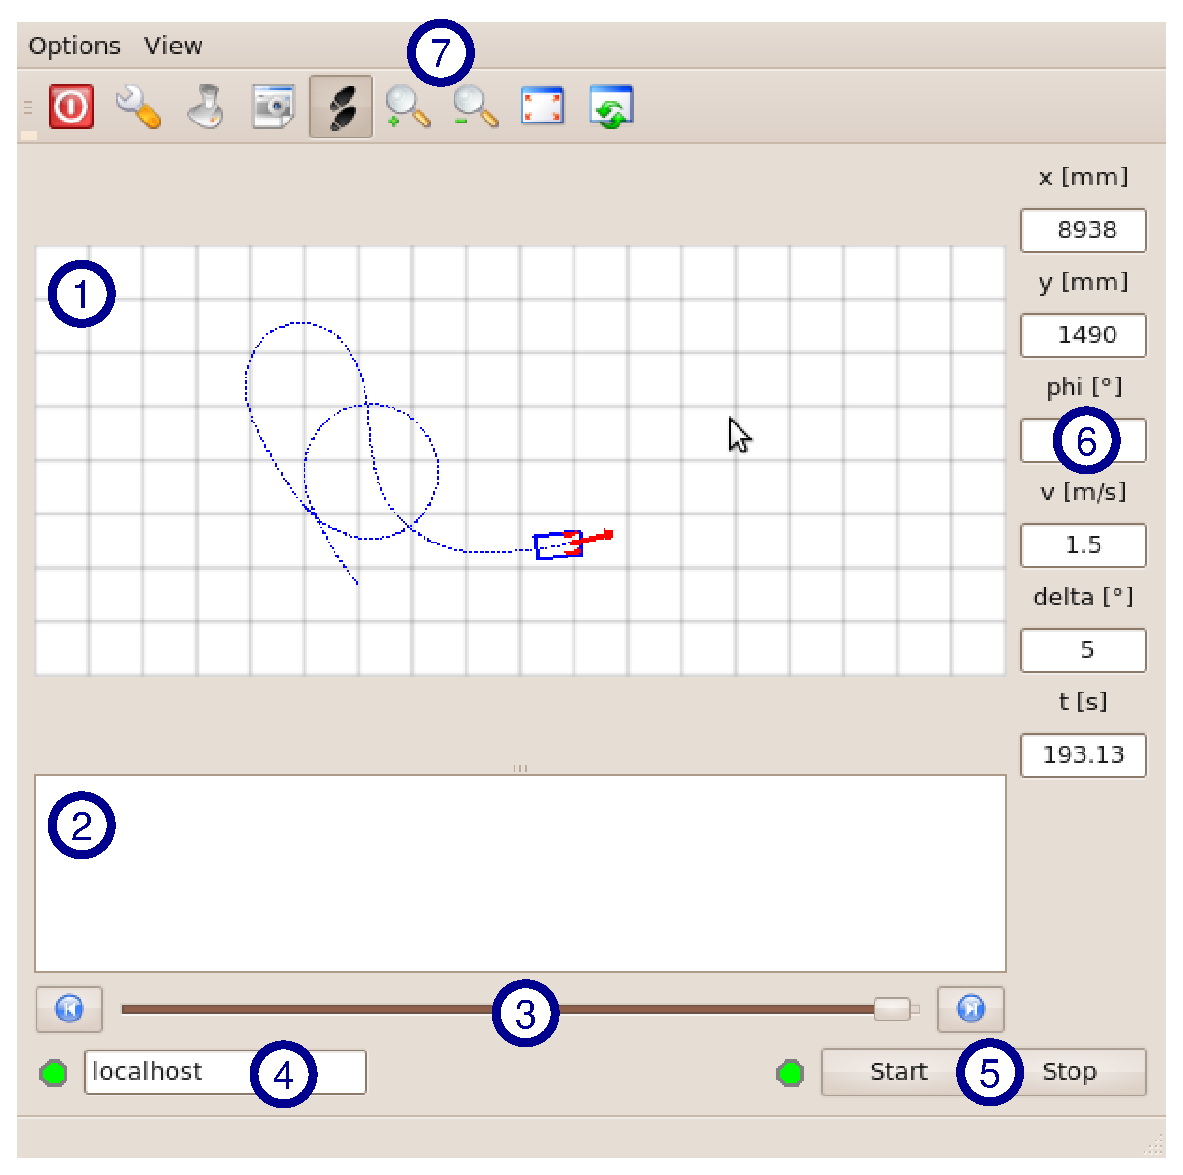
\includegraphics[width=0.8\textwidth]{anicarviewer} 
\caption{A screenshot of the \textit{AnicarViewer} GUI. Fields 1 through 7 are explained in the text.}
\label{fig:AnicarViewerSnapshot}
\end{figure}

Field (1) shows a stylised (top) view of the course. Information gained from this area includes: the current position of the vehicle (blue square), current steering angle (red line), current speed (red arrow) and , if applicable, the trajectory leading up to the present state. A click on the magnifying glasses (7) allows the user to zoom in and out on the scene. The buttons on the right of the magnifying glasses will rotate the course's view $90^\circ$. The footsteps icon will toggle the display of the trajectory on and off. The checkered background in (1) represents a regular grid of one meter distances between each parallel line. 

Field (2) is where textual messages are displayed after being processed and transmitted by \DerWeg. These messages originate in the Blackboard and can be written using the \code{addMessage()} method within the Blackboard. The message is then transmitted to \AnicarViewer automatically. These messages can be used to generate control and debugging messages, and thus to succesfully monitor the operation of \DerWeg during its runtime. 

Similar to the messages in (2), \AnicarViewer allows the user to plot simple geometrical shapes on the \DerWeg top view plot (1). To achieve this, the \code{addPlotCommand()} Blackboard method must be used. These plotting commands are formed by a specific keyword and a variable number of arguments, which are always separated by blank spaces. It is possible to enter multiple plotting commands in a row. For example, the string \texttt{\"{}thick yellow line 1000 2000 4000 2000 5000 3000 green dot 0 0\"{}} creates two objects. Here, a thick yellow polyline (or polygonal chain), with vertices at $(1000, 2000)$, $(4000,2000)$ and $(5000,3000)$, as well as a green dot with the coordinates $(0,0)$ are plotted. A list of all commands necessary to create such shapes can be found in table \ref{tab:plotcmd}.

\begin{table}
\centering
\begin{tabular}{|p{7cm}|p{8cm}|}
\hline
Command & Meaning \\
\hline
thick & plot using thick lines \\
thin & plot using thin lines \\
\hline
solid & plot using solid lines \\
dashed & plot using dash lines \\
dotted & plot using dotted lines \\
\hline
black, white, lightGray, gray, darkGray, red, darkRed, green, darkGreen, blue, darkBlue, yellow, darkYellow, cyan, darkCyan, magenta, darkMagenta & use the respective color \\
\hline
dot $x_1\;y_1\;x_2\;y_2\;\dots$ & plots dots with the coordinates: $(x_1,y_1)$, $(x_2,y_2)$ etc. \\
cross $x_1\;y_1\;x_2\;y_2\;\dots$ & plots diagonal crosses with the coordinates: $(x_1,y_1)$, $(x_2,y_2)$ etc. \\
plus $x_1\;y_1\;x_2\;y_2\;\dots$ & plots plus signs with the coordinates: $(x_1,y_1)$, $(x_2,y_2)$ etc. \\
line $x_1\;y_1\;x_2\;y_2\;x_3\;y_3\dots$ & plots a polyline using the given vertices. \\
arrow $x_1\;y_1\;x_2\;y_2$ & plots an arrow from $(x_1,y_1)$ to $(x_2,y_2)$ . \\
\hline
\end{tabular}
\caption{List of all plotting commands}
\label{tab:plotcmd}
\end{table}

The slide bar (or slider) allows us to observe the vehicle's history. Its range can be interpreted as a time axis, with the starting point on the far left of the bar, and the current point on the right. \AnicarViewer stores the vehicle's position and messages for all points in time within these parameters. By sliding the bar to the left, the user can go to an earlier point in time in order to visualize past events. It is also posible to reproduce the vehicle's behavior on a step-by-step basis. Pressing the "`n"' (next) key makes the bar go a step forward, while "`p"' (previous) makes one step backwards in time.

Field (4) shows with which computer \AnicarViewer is connected at a given point. If a connection has successfully been established, (i.e. there is an available computer, a connection has been made, and \DerWeg has been started), then the dot on the left is green. Otherwise, it will be red. Pressing the start or stop button (5) performs the respective action, (similar to using  "`g"' and "'\!$<$\!blank\!$>$\!"' in the TUI). The dot on the left will turn green when the vehicle has been started, and red when it has not.

The display bar on the right side (6) gives information regarding the current vehicle position, target speed, target angle, as well as the system time. 

\AnicarViewer also enables the use of a joystick to control the vehicle. To configure it, one must first connect the peripheral to the computer running \AnicarViewer, and subsequently press the button with the joystick symbol on the upper edge of the program window (7). Clicking the camera symbol instructs the program (\DerWeg) to save an image from the camera, which can be viewed at the end of the test drive. By clicking the wrench icon, the programm will display the modules used by \DerWeg, and will also allow the user to edit them. \footnote{Changes made her will only affect the programm that has already been started, but not to the configuration file itself.}

Aside from monitoring the test in real time, \AnicarViewer also offers the possibility to analize data at a later point in time after it has concluded. To do this, the programm creates a logfile with the name \textit{anicarviewer.log}. This logfile contains all information gathered by \AnicarViewer from \DerWeg. When starting \AnicarViewer using \texttt{./AnicarViewer -l logfile}, the programm will read all data from the logfile instead of attempting to connect with \DerWeg. Only then is it possible to view once again the course of the test drive with \AnicarViewer and analyze important situations offline. 

\subsection{Using \DerWeg}

\subsubsection{Initial Setup}

Installing the software takes the following steps: First, a command-line interface must be opened. Then, change into the directory \texttt{KognitiveAutomobileLabor/} and enter the following command:
\begin{quote}
make install
\end{quote}

\subsubsection{Starting the Program}

The Program \DerWeg can be started using a command-line interface and invoking: \texttt{./DerWeg} or \texttt{./DerWeg Konfigurationsdatei}. \texttt{Konfigurationsdatei} is the name of a configuration file that contains information about the available software modules, as well as other parameters relevant to them. If no configuration file is specified, the computer will load the default file called \textit{default.cfg}. A call for \DerWeg should always proceed from the \texttt{bin-/} directory in order to find the correct configuration file. 

Upon starting, the program will attempt to initialize the selected modules. If necessary, debug output will be written in the console. After all modules have been initialized, each individual module will start to run. (This means that the \code{execute()} function will be called for each module in form of a thread). If the programm fails to initialize all modules, \DerWeg will display an error message and abort.

Note: Should the software work with stereoscopic image processing, it should be started from the laptop using \textit{optirun}. To do so, it is convenient to start optirun using the \texttt{optirun bash} command on the command-line. Afterwards, \DerWeg can be started as usual.

\subsubsection{Configuration File}
\label{sec:config}

The configuration file contains a description of the modules to be started, as well as other other parameters relevant to each of them. The file is built based on the \textit{Key-value store} paradigm, i.e. all lines have one of the following forms:
\begin{quote}
Keyword = Value\\
Keyword = Value1 Value2 Value3 ...
\end{quote}
Comments are started with the hash symbol (\#). In the following examples, the compiler would ignore the areas marked with a XXX. 
\begin{quote}
\# XXX\\
Keyword = Value \# XXX
\end{quote}

In order to better define keywords without any conflict, it is possible to divide them into sections and put them under headings. To create a heading, its name should simply be written in square brackets. For example:
\begin{quote}
\mbox{}Keyword1 = Value1 \\
\mbox{}[Heading1] \\
\mbox{}Keyword2 = Value2 \\
\mbox{}Keyword3 = Value3 \\
\mbox{}[Heading2] \\
\mbox{}Keyword4 = Value4
\end{quote}
In this case \textit{Keyword1} does not sit under any heading, \textit{Keyword2} and \textit{Keyword3} both sit under \textit{Heading1}, and \textit{Keyword4} is under \textit{Heading2}. When the \code{ConfigReader} reads the file, it sets the heading in front of the keyword and divides them via a double column \texttt{::}. In the above example, the complete keywords would be defined as \textit{Keyword1}, \textit{Heading1::Keyword2}, \textit{Heading1::Keyword3}, and \textit{Heading2::Keyword4}.

The +-symbol lets you include additional configuration files recursively. For example, the following line includes the \textit{landmarks.cfg}:
\begin{quote}
+ landmarks.cfg
\end{quote}

In order to attain an easily understandable configuration file that is free of conflict, the following conventions must be always be followed.
\begin{itemize}
\item The key word \textit{Modules} (without heading) is reserved for the list of modules to be started.
\item Parameters that are relevant for a given XXX module, should sit under the homonymous header. 
\item Parameters that belong to the same module should be written close together.
\item All parameters should be given self-explanatory names and, if necessary, should be explained using comments.
\end{itemize}

The \textit{default.cfg} file already contains an executable configuration, which can be directly used on the vehicle. 

\subsubsection{Available Modules}
\label{sec:modules}

The software's base configuration comes with some preinstalled modules. These modules include basic functions such as camera and motor controls, but also examples of image processing and vehicle control systems. A list of these basic modules can be found in table \ref{tab:modules}.

\begin{table}
\centering
\begin{tabular}{p{0.24\textwidth}p{0.7\textwidth}}
\hline
Name & Functionality \\
\hline\hline
\multicolumn{2}{|c|}{\textsc{Localization Modules:}} \\
\hline
TopGigE & \raggedright Camera driver for the localization camera. Essential for localization. \tabularnewline
CameraLocalization & \raggedright Localization with use of landmarks. Additionally requires the TopGigE module. \tabularnewline
%StarGazerGyro & \raggedright Localization using landmarks and gyroscope. Works only for AniCar with enabled StarGazer and tethered inertial measuring unit  \tabularnewline
%StarGazerOnly & \raggedright Localization using landmarks. Works only for AniCar with enabled StarGazer \tabularnewline
DeadReckoning & \raggedright Localization using DeadReckoning. That is, by integrating its odometry. \tabularnewline
ShowLocalization & \raggedright Graphically displays the driven path on the screen. \tabularnewline
\hline
\multicolumn{2}{|c|}{\textsc{Modules related to Camera \& Images:}} \\
\hline
%GigE & \raggedright Monoscopic camera driver. Possesses options for selecting display detail, white balance, and auto-exposure. \tabularnewline
StereoGigE & \raggedright Camera driver for the stereoscopic camera system. Apart from that, analog to GigE \tabularnewline
ImagesFromFile & \raggedright Loads saved images from the hard disk. Image index and filenames can be accessed using additional parameters in the configuration file. This module can be used for testing and debugging as an alternative to GigE.  \tabularnewline
SaveCameraImages & \raggedright Saves all incoming images on the hard disk. Index and filenames can be defined in the configuration file. This module is suitable for recording image sequences. \tabularnewline
ShowCameraImages & \raggedright Displays approx. 2 images or 2 image pairs per second on the screen.\tabularnewline
ShowStereo \hspace*{2em}\mbox{CameraImages} & \raggedright Displays approx. two stereo image pairs per second, as well as the approximated disparity between them. \tabularnewline
\hline
\multicolumn{2}{|c|}{\textsc{Modules related to Motor Control:}} \\
\hline
MotorInterface & \raggedright Controls for the steering and driving motors on the AniCar. These parameters should not be modified. \tabularnewline
MotorDummy & \raggedright A dummy motor control that does nothing but records the desired speed and rewrites it as odometry on the Blackboard. Serves as an alternative to MotorInterface when AniCar is not in use. \tabularnewline
AnicarSimulation & \raggedright A simulator. It simulates vehicle behavior and, in the process, partially considers the effects of disruptions as well. When simulating, this module replaces the motor control module, as well as the localization module.  \tabularnewline
\hline
\multicolumn{2}{|c|}{\textsc{Modules related to the User Interface:}} \\
\hline
TUI & \raggedright Command-line interface, see section \ref{sec:tui}. Should always be selected. \tabularnewline
AnicarViewer & \raggedright Graphical User Interface. See section \ref{sec:gui}. Should always be selected. \tabularnewline
\hline
\end{tabular}
\caption{Preinstalled Modules}
\label{tab:modules}
\end{table} ShowStereoCameraImages

These modules allow us to make some useful combinations from the beginning. Should you wish to let the vehicle drive in a fully autonomous mode, you would need, at least, the MotorInterface, TopGigE, CameraLocalization, StereoGigE, TUI, and AnicarViewer modules. If, on the other hand, you wanted to carry out a manually controlled testdrive (e.g. with a joystick), and wanted to record camera images, then the MotorInterace, GigE, TUI, AnicarViewer, and SaveCameraImages modules would be useful. Furthermore, if the images were to be copied into a PC, and we wished to replay the testdrive afterwards, one way we to do so would be by starting \DerWeg using ImagesFromFile, TUI, Anicarviewer, and ShowCameraImages. Thereby it is possible, for instance, to test an image processing algorithm until it is possible to work with the images and no errors. When planning paths, as well as longitudinal and transverse regulating processes, it would be sensible to combine the modules TUI, AnicarViewer und AnicarSimulation.

In addition to the basis modules, \DerWeg contains the vehicle control modules \textit{StopAtRed}, %\textit{StopAtNoentry},
\textit{DriveWigglyLines} and \textit{CyclicForwardsBackwards}. These modules serve as an example of how simple vehicle behavior can be generated. The source code for these three modules can be found in the Annex \ref{app:codeexamples} of this document. 

StopAtRed carries out a simple image evaluation. It counts how many of the pixels in a camera image are red. Should this number be higher than a given threshold value, the car is stopped. Otherwise, it continues on its path. This module combines very simple image processing  and the influence target-speed values have on it. Vehicle localization is not needed in this case. Should one wish to observe what the vehicle behavior would look like here, \DerWeg should be started using the combination MotorInterface, StereoGigE, TUI, GUI, StopAtRed.

%StopAtNoEntry is a variation of StopAtRed. It employs the road sign identifiers described in section \ref{sec:gegebene_funktionen}, instead of counting red pixels. This module can be tested using the module combination MotorInterface, GigE, TUI, GUI, StopAtNoEntry.

The second demo application implements a very straightforward controller in order to follow the $y=2000$ line. Here, the steering angle will be adjusted proportionally to the distance of the vehicle to the target line. If the vehicle is situated more than 1.5 m from the line, the vehicle will stop. This module combines vehicle localization with a very simple steering control system. Camera images are not needed. Thus, one can manage only by using the MotorInterface, TopGigE, CameraLocalization, TUI, GUI, and DriveWigglyLines modules.

The third application, CyclicForwardsBackwards, performs without using image processing or localization. It works by alternating the driving motor between a forwards and a backwards movement, and steers left and right in the same fashion, hence creating a star-shaped path. This program is an example of a vehicle control system that works without the need of feedback.

\textit{Please note the following:} As previously stated, the three demo applications are very simple programs and will not detect when the vehicle leaves the track. That is why someone should always sit and monitor \AnicarViewer, so he/she can push "`Stop"' if necessary!

\section{Development Environment (IDE)}

\subsection{Linux Operating System}

The software was developed using Linux. Although to some people Linux can take some time getting used to, it is in essence no harder to operate than Windows. He who prefers to work by "`clicking"', should have no problem finding sufficient software tools in Linux to work with. The advantage that Linux has over windows is that it offers some alternatives to "`drag-and-drop"' and "`clicking"', which after some familiarization, prove to be highly efficient. 

In contrast to Windows, the Linux terminal (which is similar to the DOS window in Windows) plays a huge role. From this window, it is possible to browse through the directory structure of the file system and even start programs. To start a program with the terminal, the name of the programm should simply be entered; in some cases, preceded by a "`./"'. There are several editors that can be used to edit text files. Some of these are: \textit{kate}, \textit{gedit}, \textit{joe}, and \textit{vi}. (The last two items are somewhat harder to operate).

We have already installed a basic Linux-based program  on the Anicar and regular PCs that should be enough for the vast majority of scenarios. If something is missing, please notify us and we will install it.

\subsection{Programming language C++}

The \DerWeg software is written in the C++ programming language. C++ is one of the most widely used programming languages in the world and is very suitable for time sensitive, low-level applications (as opposed to Java). Syntax is to Java, and adapting should not present any considerable difficulties for a Java programmer. A C++ tutorial from Lutz Frommberger is available at \texttt{http://www.aussagekraft.de/files/c-intro-handout.pdf}.

\subsection{Development Environment (IDE)}

There is a great variety of development environments available for Linux. However, we currently only support \textit{Code::Blocks}. Anyone who has already worked with the Visual-IDEs will realize that there is much in \textit{Code::Blocks} that they already know. (See section \ref{fig:codeblockssnapshot}). The project file is named \textit{DerWeg.cbp}.

For those who think integrated development environments are too complicated for them are also free to program with ordinary text editors or any other development environment. To make this possible, we have set up a makefile that evaluates the \textit{Code::Blocks} project files and interprets the software. Should one wish to add additional files to the project, it can be done by adding them to the \textit{Code::Blocks}- project files.

\begin{figure}
\centering
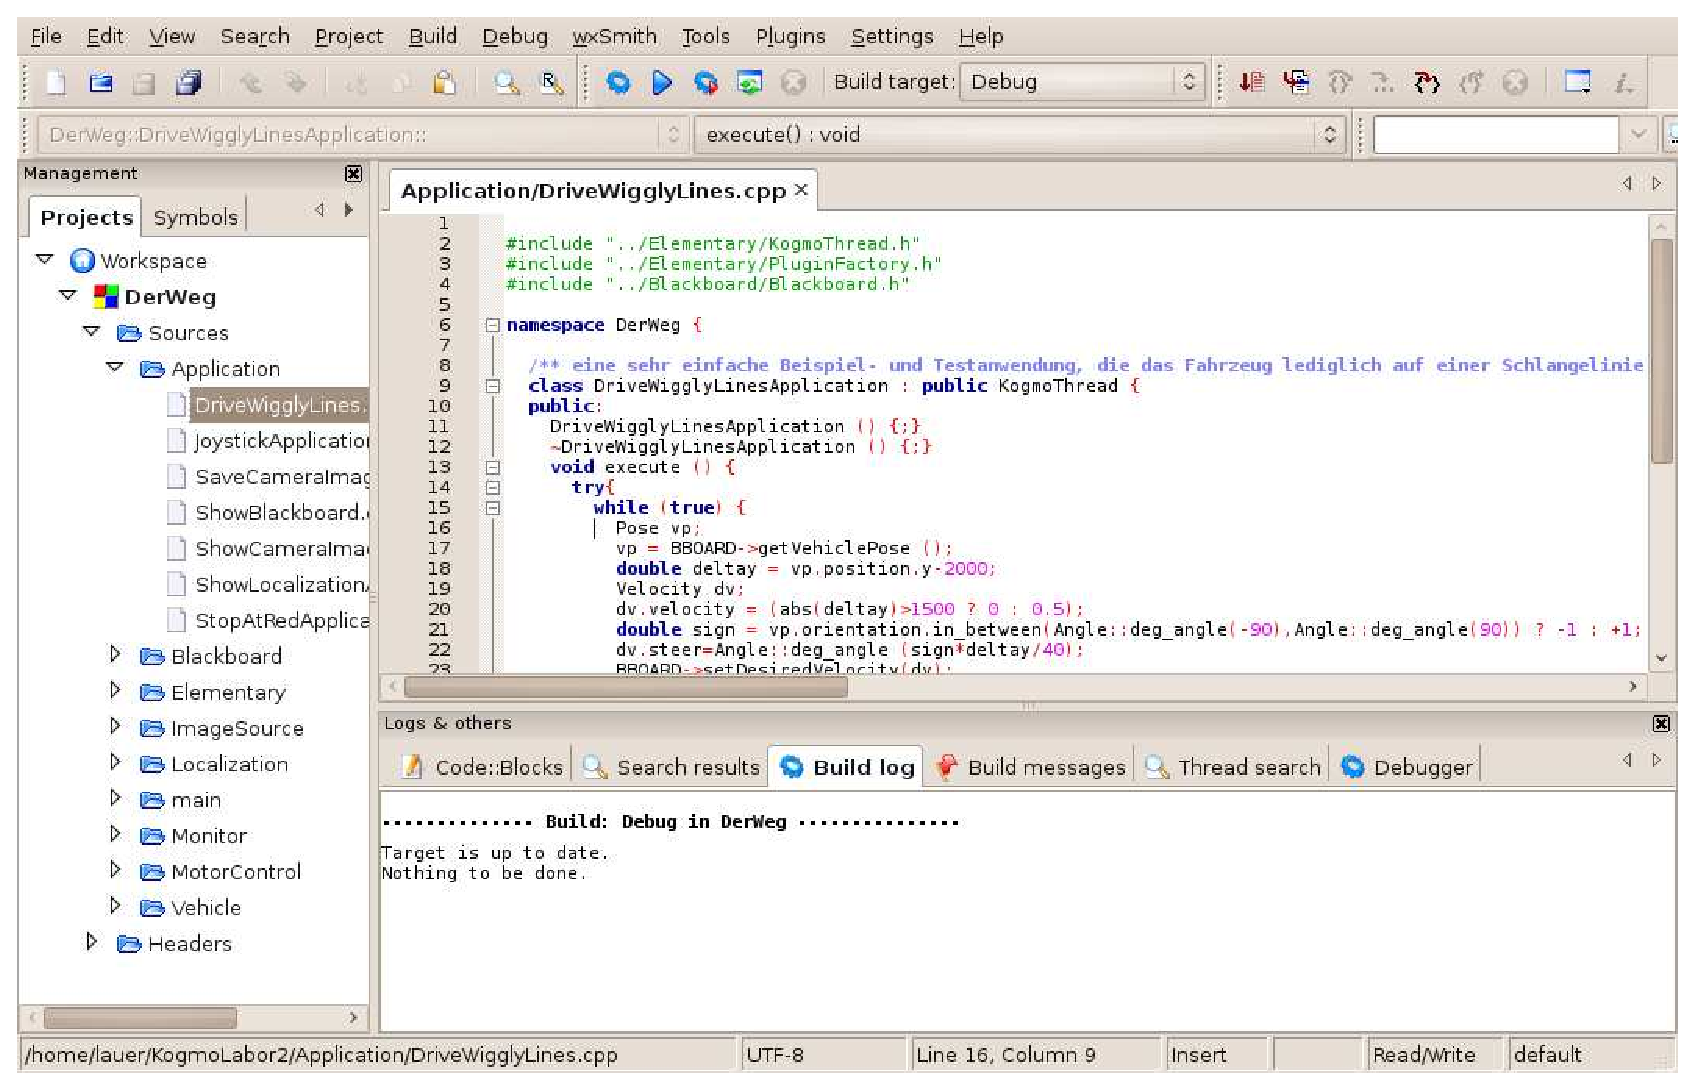
\includegraphics[width=0.8\textwidth]{codeblockssnapshot}
\caption{A snapshot of the development environment.}
\label{fig:codeblockssnapshot}
\end{figure}

Tips for a proper use of \textit{Code::Blocks}: 
\begin{itemize}
\item Adding source files: If a source file is added to a project within Code::Blocks, it is important to save the project file using (Menu$\rightarrow$File$\rightarrow$Save project). Otherwise, the new file will not be interpreted.
\item Should you wish to interpret the software on a computer that does not have Cuda support, on which the camera drivers are not working, or that carries an old version of opencv, it is possible to switch by selecting \textit{Build target}. The \textit{nostereo} option ignores the stereo image processing portion, and the \textit{nocamera} option ignores camera drivers including stereo image processing.
\end{itemize}

\subsection{Software Upgrades}

Given that \DerWeg was developed just-in-time, one should not ignore the fact that we might still eventually deliver some additional bugfixes and/or enhancements. To facilitate this, the following conventions should be followed: The framework program of \DerWeg and the modules that are part of the basic configuration are only to be serviced by the lab staff. Alterations made by participants are not allowed. However, participants are responsible for all programs and modules that supplement the basic software.

However severe these regulations might sound, they are necessary in order to maintain the consistency of the software. Even if it were to feel logical to edit parts of the basic software, it is the wrong course of action. If you find any bugs on parts of the software, please let a supervisor know. If you experience problems due to missing functionality, please report to your supervisor first. If the preexisting demo modules serve as a good basis for further development, please copy the needed modules, rename them, and edit only the copied version.

\subsection{Versioning Control System}

When developing software in a team, it is exceptionally helpful to use a versioning control system that manages all different software files, stores old versions, and merges changes made by multiple developers. Therefore, we provide each group with an SVN repository. All changes made on the base software will also be provided on the aforementioned repository. 

Based on previous experience, we highly recommend the use of the SVN repositories. Initially, they seem to create some unnecessary overhead. However, the naive method of data exchange by means of e-mail and USB sticks will turn cumbersome after just a few weeks.

\subsection{Program Documentation}

The program code is prepared to create HTML documentation with help of \textit{doxygen}. To generate said documentation, one must only access the project folder on the console and invoke \texttt{doxygen} from there. The HTML documentation will be created in the subfolder \textit{doc/html} and can be viewed on any browser. 

This document is located in the \textit{doc/SoftwareDoku} subfolder and can be created by calling \texttt{pdflatex softwaredoku}.

\appendix

\section{Appendix: Blackboard Public Interface}
\label{app:blackboard}

\codeex{blackboardInterface.h}

\section{Annex: Code Examples}
\label{app:codeexamples}

\codeex{DriveWigglyLines.cpp}
\pagebreak

\codeex{StopAtRed.cpp}
\pagebreak

%\codeex{StopAtNoEntry.cpp}
%\pagebreak

\codeex{CyclicForwardsBackwards.cpp}


\end{document}
